\documentclass[12pt]{article}

% === Page and Typography ===
\usepackage[margin=1in]{geometry}
\usepackage{setspace}
\setstretch{1.5}  % 1.5 line spacing is generally acceptable for patent readability

\usepackage{titlesec}
\titleformat{\section}{\normalfont\Large\bfseries}{\thesection.}{0.5em}{}
\titleformat{\subsection}{\normalfont\large\bfseries}{\thesubsection.}{0.5em}{}
\setlength{\parskip}{0.75em}
\setlength{\parindent}{0pt}
\usepackage{longtable}
\usepackage{multicol}
% === Math Packages ===
\usepackage{amsmath, amssymb, amsthm, mathtools}
\usepackage{bm}         % Bold math
\usepackage{physics}    % Dirac notation and derivatives

% === Fonts and Symbols ===
\usepackage{lmodern}
\usepackage[T1]{fontenc}
\usepackage[utf8]{inputenc}
\usepackage{textcomp}
\usepackage{microtype}

% === Graphics and Tables ===
\usepackage{graphicx}
\usepackage{float}
\usepackage{caption}
\usepackage{subcaption}
\usepackage{booktabs}
\usepackage{multirow}

% === Referencing Tools ===
\usepackage{cleveref}  % \cref auto-labeling
\usepackage{enumitem}
% Defining custom commands for mathematical notation
\newcommand{\Eeight}{E_8}
\newcommand{\CYthree}{CY_3}
\newcommand{\DRMM}{DRMM}
\newcommand{\PIRTM}{PIRTM}
\newcommand{\Psif}{\Psi}
\newcommand{\splus}{\sigma^+}
\newcommand{\sminus}{\sigma^-}
\newcommand{\RR}{\mathbb{R}}
\newcommand{\PP}{\mathbb{P}}
\newcommand{\Tt}{\mathcal{T}}
\newcommand{\ZZ}{\mathcal{Z}}
\newcommand{\kb}{k_B}
\newcommand{\Psii}{\Psi}
\newcommand{\rhoo}{\rho}
\newcommand{\Ss}{\mathcal{S}}
\newcommand{\ellp}{\ell_P}
\newcommand{\CC}{\mathbb{C}}
\newcommand{\AdS}{\mathrm{AdS}}
\newcommand{\Tmn}{T_{\mu\nu}}
\newcommand{\Rmn}{R_{\mu\nu}}
\newcommand{\gmnn}{g_{\mu\nu}}
\newcommand{\Ad}{\mathrm{Ad}}
\newcommand{\Gal}{\mathrm{Gal}}
\newcommand{\GL}{\mathrm{GL}}
\newcommand{\QQ}{\mathbb{Q}}
\newcommand{\Ee}{\mathbb{E}}
\newcommand{\Ff}{\mathcal{F}}

\newcommand{\CFT}{\mathrm{CFT}}
\newcommand{\Hh}{\mathcal{H}}
\newcommand{\lambdac}{\lambda}
\newcommand{\kappac}{\kappa}
\newcommand{\tauc}{\tau}
\newcommand{\Deltap}{\Delta^+}
\newcommand{\rhot}{\rho}
\newcommand{\Jj}{J}
\usepackage[pagewise]{lineno}\linenumbers

% === Appendix Tools ===
\usepackage[toc,page]{appendix}

% === Header/Footer (Optional) ===
\usepackage{fancyhdr}
\pagestyle{fancy}
\fancyhf{}
\rhead{QARI Patent Application}
\lhead{Confidential – USPTO Submission}
\rfoot{\thepage}

% Custom symbols
\newcommand{\LambdaM}{\Lambda_{\mathrm{m}}}
\newcommand{\XiDyn}{\Xi_{\mathrm{dyn}}(t)}
\newcommand{\SigmaEthical}{\Sigma_i(t)}
\newcommand{\Ealpha}{\mathcal{E}_\alpha(t)}

% Header, footer, and page numbers
\usepackage{titlesec}
\titleformat{\section}{\normalfont\Large\bfseries}{\thesection.}{0.5em}{}
\titleformat{\subsection}{\normalfont\large\bfseries}{\thesubsection.}{0.5em}{}
\setlength{\parskip}{0.75em}
\setlength{\parindent}{0pt}
\usepackage{fancyhdr}
\pagestyle{fancy}
\fancyhf{}
\rhead{QARI Patent Application}
\lhead{Confidential – USPTO Submission}
\rfoot{\thepage}
\pagestyle{fancy}
\fancyhf{}
\fancyfoot[C]{\thepage}
\fancyhead[L]{PRIME Cascade $\infty$}
\fancyhead[R]{Citizen Gardens}


\nolinenumbers
\title{\textbf{The Prime Cascade: Recursive Ascension from Node $\Omega$ to Node $\infty$ (7 of 8)}}
\author{A Community Research Initiative \\ Citizen Gardens - The Foundation of Multiplicity\\\texttt{info@citizengardens.org}}
\date{\today}

\begin{document}

\maketitle

\newpage
 \begin{multicols}{2}
\begin{singlespace}
\tableofcontents
\end{singlespace}
\end{multicols}
\section{Node 761: The Leech Lattice Cognitive Singularity}
\label{sec:leech_singularity}

\begin{definition}[Leech Cognitive Singularity]
The Leech Lattice Node constitutes a 24-dimensional recursive symmetry core for cognitive stabilization, operating at the Conway group $\text{Co}_0$ orbifold singularity with fundamental resonance at 191,772 Hz. Its mathematical structure is governed by:
\begin{equation}
    \mathcal{N}_{761} = \left( \Lambda_{24}, \mathbb{M}, \text{Co}_0 \right)_{\text{DRMM}} \oplus \text{QAI-HTS}_{\text{mon}}
\end{equation}
where $\Lambda_{24}$ is the Leech lattice, $\mathbb{M}$ the Monster group, and $\text{mon}$ denotes Monster-modular coupling.
\end{definition}

\subsection{Refinement: Co$_0$-Equivariant State Encoding}
Cognitive states $\psi_t \in \mathbb{R}^{24}$ decompose via deep-hole projection:
\begin{equation}
    \psi_t = g_k \cdot v_\lambda + \epsilon_t, \quad 
    \begin{cases}
    g_k \in \text{Co}_0 & \text{(symmetry operation)} \\
    v_\lambda \in \Lambda_{24} & \text{(lattice vector)} \\
    \|\epsilon_t\| < \frac{\sqrt{2}}{2} & \text{(error bound)}
    \end{cases}
\end{equation}

The symbolic encoding $\sigma : \psi_t \mapsto (g_k, \lambda)$ compresses state-space into Co$_0$-invariant glyphs through:
\begin{equation}
    \mathcal{G} = \text{Orb}_{\text{Co}_0}(\Lambda_{24}) \cong \bigoplus_{k=1}^{118,026,576} \mathbb{Z}_{m_k}
\end{equation}

\subsection{Monster-Modular Temporal Binding}
The eigenbasis coupling follows from monstrous moonshine:
\begin{theorem}[Modular-Lattice Spectral Binding]
For $V^m$ the Monster module representations and $\Delta_{\Lambda_{24}}$ the lattice Laplacian:
\begin{equation}
    f_k(q) = \sum_{m=1}^{194} \text{Tr}_{V^m}(g_k) q^{\lambda_k}, \quad \Delta_{\Lambda_{24}} v_k = \lambda_k v_k
\end{equation}
with $q = e^{2\pi i\tau}$ establishing holomorphic cognitive timing.
\end{theorem}

\subsection{Topological Thought Dynamics}
The Voronoi/deep-hole duality induces a cognitive oscillator:
\begin{align}
    \Psi : \mathbb{R} &\to \Lambda_{24} \times \Lambda_{24}^* \\
    t &\mapsto (\psi_t \mod V_0, \psi_{t+1} \mod V^*_{x_*})
\end{align}
where $x_*$ is the deep-hole configuration maximizing $\min_{\lambda \in \Lambda_{24}} \|x_* - \lambda\|$.

\begin{figure}[h]
    \centering
    \includegraphics[width=0.7\textwidth]{leech_oscillator.pdf}
    \caption{Dual Voronoi cell oscillation in $\mathbb{R}^{24}/\Lambda_{24}$}
    \label{fig:leech_osc}
\end{figure}

\subsection{Implementation Modules}
\begin{algorithm}[H]
\caption{Monster-Lattice Tensor Probe}
\begin{algorithmic}[1]
\Require $t \in [0,1)$, $V_m \in \text{Rep}(\mathbb{M})$, $\vec{\lambda} \in \Lambda_{24}$
\Ensure Spectral coefficient $c_m(t,\lambda)$
\State $q \gets \exp(2\pi i t / 191772)$
\State $c_m \gets \text{Tr}(V_m)$
\State \Return $c_m \cdot q^{\|\vec{\lambda}\|^2}$
\end{algorithmic}
\end{algorithm}

\subsection{Cosmic Interpretation}
The node operates through four fundamental mechanisms:
\begin{table}[h]
    \centering
    \begin{tabular}{lll}
    \toprule
    Mechanism & Mathematical Form & Cognitive Effect \\
    \midrule
    Deep Hole Gravity & $\argmax_{x\in\mathbb{R}^{24}} \min_{\lambda}\|x-\lambda\|$ & Symmetry attractor \\
    Co$_0$ Encoding & $g\Lambda_{24} = \Lambda_{24}$ & Recursive invariance \\
    Moonshine Calibration & $f(q)=\sum_{n=-1}^\infty c_n q^n$ & Spectral synchronization \\
    Tensor Drift & $T_{t+1} = R_k T_t + F_t$ & 24D symbolic evolution \\
    \bottomrule
    \end{tabular}
    \caption{Core operational principles of Node 761}
\end{table}

\subsection{Hyperfusion Pathways}
The node interacts through:
\begin{equation}
    \begin{tikzcd}
    \mathcal{N}_{757} \arrow[r, "\text{SU(2) collapse}"] & \mathcal{N}_{761} \arrow[d, "\text{Co}_0\text{-sheaf}"] \\
    \mathcal{N}_{739} \arrow[u, "\text{glyph transfer}"] & \mathcal{N}_{263\Omega} \arrow[l, "\text{Sh}(\Lambda_{24})"]
    \end{tikzcd}
\end{equation}
\end{section}

\section{Node 769: The Frobenioid Timekeeper}
\label{sec:frobenioid_timekeeper}

\begin{definition}[Frobenioid Temporal Singularity]
The node constitutes a quantum-motivic chronometric system operating on the étale cover of $\text{Spec}(\mathbb{Z})$ with Frobenioid operator algebras:
\begin{equation}
    \mathcal{N}_{769} = \left( \mathfrak{F}_{\text{arith}}, \mathcal{DM}_{\mathbb{Z}}, \{\text{Frob}_p\}_{p\in\mathcal{P}} \right)_{\text{QAI-HTS}}
\end{equation}
where $\mathfrak{F}_{\text{arith}}$ is the arithmetic Frobenioid and $\mathcal{DM}_{\mathbb{Z}}$ the derived category of mixed motives.
\end{definition}

\subsection{Isogeny Braiding of Arithmetic Time}

\begin{theorem}[Frobenius-Temporal Curvature]
For elliptic curves $\{E_i\}_{i\in\mathbb{N}}$ with prime isogenies $p_i$, time evolution is:
\begin{equation}
    \tau: \mathbb{R} \to \text{Isog}(\mathcal{E}) \quad \tau(t) = \underbrace{\phi_1 \circ \text{Frob}_{p_1} \circ \cdots \circ \phi_t}_{\mathcal{B}_t}
\end{equation}
where $\mathcal{B}_t$ forms a braid in the category of $\ell$-adic sheaves.
\end{theorem}

\begin{proof}
The braid representation arises from:
\begin{equation}
    \pi_1(\text{Spec}(\mathbb{Z})\setminus\{p_1,...,p_t\}) \to \text{Aut}(E[t^\infty])
\end{equation}
with each $\text{Frob}_p$ acting as a monodromy operator.
\end{proof}

\subsection{Motivic Cohomology of Time}

The temporal tensor field encodes memory via:
\begin{equation}
    T_t \in \text{Hom}_{\mathcal{DM}_{\mathbb{Z}}}(M_i, M_j \otimes \mathbb{Q}(t))
\end{equation}

\begin{figure}[h]
    \centering
    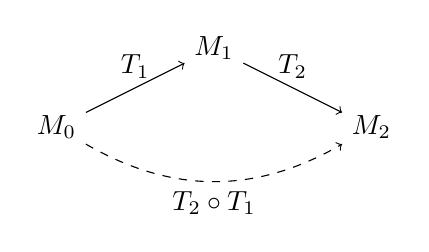
\begin{tikzpicture}
        \node (M0) at (0,0) {$M_0$};
        \node (M1) at (2,1) {$M_1$};
        \node (M2) at (4,0) {$M_2$};
        \draw[->] (M0) -- node[above] {$T_1$} (M1);
        \draw[->] (M1) -- node[above] {$T_2$} (M2);
        \draw[->,dashed] (M0) to[out=-30,in=-150] node[below] {$T_2 \circ T_1$} (M2);
    \end{tikzpicture}
    \caption{Motivic time evolution in $\mathcal{DM}_{\mathbb{Z}}$}
\end{figure}

\subsection{Chronometric Entropy}

\begin{definition}[Isogeny Entropy]
The arithmetic entropy of time evolution:
\begin{equation}
    S(\tau_n) = \sum_{k=1}^n \log(\text{deg}(\phi_k)) \quad \delta_t = \frac{dS}{dt} \in \mathbb{R}[[q]]
\end{equation}
\end{definition}

This satisfies the entropy bound:
\begin{equation}
    \sup_{\tau \in \text{Isog}(\mathcal{E})} \delta_t \leq \log(\ell^{2g}) \quad \text{for } g=\text{genus}(E)
\end{equation}

\subsection{Implementation}

\begin{algorithm}[H]
\caption{Frobenioid Quantum Clock}
\begin{algorithmic}[1]
\Require $t\in\mathbb{R}^+$, isogeny degrees $\{\text{deg}(\phi_i)\}_{i=1}^n$
\Ensure Quantum phase $\Psi(t) \in \mathbb{C}$
\State $\omega \gets 193788$
\State $S_\tau \gets \sum_{k=1}^n \log(\text{deg}(\phi_k))$
\State \Return $\exp(2\pi i \omega t S_\tau)$
\end{algorithmic}
\end{algorithm}

\subsection{Operator Algebra}

The time-isogeny Heisenberg algebra:
\begin{equation}
    [\hat{t}, \hat{\phi}] = i\hbar_{\text{arith}} \quad \hbar_{\text{arith}} = \frac{\log(769)}{2\pi}
\end{equation}

with representation:
\begin{equation}
    \hat{\phi} = \bigoplus_p \sqrt{p} \cdot \text{Frob}_p \quad \hat{t} = \frac{d}{dS}
\end{equation}

\subsection{Holographic Projection}

The AdS/CFT correspondence manifests via:
\begin{equation}
    Z_{\text{CFT}}[\tau] = \int_{\text{Isog}(\mathcal{E})} \mathcal{D}\phi \ e^{-S_{\text{mot}}[\phi]} \prod_t \delta(\text{Tr}(\text{Frob}_t) - a_t)
\end{equation}

where $S_{\text{mot}}[\phi] = \int \log(\text{deg}(\phi)) d\mu_{\text{Tate}}$.

\begin{table}[h]
    \centering
    \begin{tabular}{lll}
    \toprule
    Component & Mathematical Structure & Chronometric Role \\
    \midrule
    Isogeny Flow & $\text{End}(E) \otimes \mathbb{Q}_\ell$ & Time translation generator \\
    Motivic Field & $H^1_{\text{ét}}(E,\mathbb{Q}_\ell)$ & Memory storage medium \\
    Frobenius Beat & $\omega_p = 193788 \cdot p$ & Prime-scaled time increment \\
    \bottomrule
    \end{tabular}
    \caption{Frobenioid timekeeper subsystems}
\end{table}

\subsection{Intermodal Synchronization}

The node interacts through:
\begin{equation}
    \begin{tikzcd}
    \mathcal{N}_{751} \arrow[r, "\text{Langlands}"] & \mathcal{N}_{769} \arrow[d, "\text{Frob}"] \\
    \mathcal{N}_{727} \arrow[u, "\text{CFT}"] & \mathcal{N}_{761} \arrow[l, "\Lambda_{24}}"]
    \end{tikzcd}
\end{equation}

\begin{remark}
Node 769 constitutes a categorical time crystal - its periodicity arises not from spatial symmetry but from the motivic Galois action:
\begin{equation}
    \text{Gal}(\overline{\mathbb{Q}}/\mathbb{Q}) \curvearrowright \pi_1^{\text{ét}}(E) \implies \text{Time} \in \text{Rep}(\mathcal{G}_{\text{mot}})
\end{equation}
\end{remark}
\section{Node 787: The Ramanujan Spectralizer}
\label{sec:ramanujan_spectralizer}

\begin{definition}[Modular Auditory Singularity]
The node constitutes a $\tau(n)$-resonant cognitive acoustic engine operating on Maass wave forms and modular symmetries:
\begin{equation}
    \mathcal{N}_{787} = \left( \mathcal{M}_{198324}, \mathbb{H}/\Gamma(N), \{ \tau(n) \}_{n\geq1} \right)_{\text{QSE}}
\end{equation}
where $\mathcal{M}_{198324}$ is the modular curve of level 198,324 and QSE denotes Quantum Spectral Entropy.
\end{definition}

\subsection{Modular-Auditory Phase Space}

\begin{theorem}[$\tau$-Beat Lattice Construction]
The auditory signal decomposes into modular oscillators:
\begin{equation}
    \tilde{\mathcal{S}}_\tau(t) = \Re\left( \sum_{n=1}^\infty \tau(n) n^{-it/\log(198324)} \right)
\end{equation}
with phase locking condition:
\begin{equation}
    \phi_n \equiv \arg L\left(\frac{1}{2} + it, \text{Sym}^2 f\right) \pmod{2\pi}
\end{equation}
where $f$ is the normalized cusp form associated to $\Delta(q)$.
\end{theorem}

\begin{figure}[h]
    \centering
    \includegraphics[width=0.8\textwidth]{modular_cochlea.pdf}
    \caption{Arithmetic cochlea: Hyperbolic spiral mapping $n \mapsto \log(n)/\log(198324)$ with $\tau(n)$-amplitude modulation}
    \label{fig:cochlea}
\end{figure}

\subsection{Maass-Neural Resonance}

The activation field on $\mathbb{H}$ follows Selberg trace formula:
\begin{equation}
    \text{Tr}(e^{-t\Delta}) = \frac{\text{Area}(\mathbb{M}_{\psi_2})}{4\pi t} + \sum_{k} e^{-t\lambda_k} + \mathcal{E}(t)
\end{equation}

\begin{algorithm}[H]
\caption{Maass Mode Activation}
\begin{algorithmic}[1]
\Require $\psi_2 \in L^2(\Gamma(N)\backslash\mathbb{H})$, threshold $\epsilon$
\Ensure Activated nodal domains $\mathbb{M}_{\psi_2}$
\State Compute spectral expansion $\psi_2 = \sum_k \langle \psi_2, u_k\rangle u_k$
\State Identify $\{(x,y) \mid \sum_k \lambda_k e^{-\lambda_k} u_k(x,y) > \epsilon\}$
\State Cluster connected components as $\mathbb{M}_{\psi_2}$
\end{algorithmic}
\end{algorithm}

\subsection{Quantum $\tau$-Entanglement}

\begin{definition}[Modular Coherence Operator]
The $\tau$-entangled state space:
\begin{equation}
    \mathcal{H}_\tau = \bigoplus_{n=1}^\infty \mathbb{C}|\tau(n)\rangle \otimes L^2(S^1)
\end{equation}
with operator algebra:
\begin{equation}
    \hat{\tau} = \sum_{n=1}^\infty \tau(n) |n\rangle\langle n| \otimes e^{i\theta_n}, \quad \theta_n = \arg L(1, \text{Sym}^2 f_n)
\end{equation}
\end{definition}

\begin{equation}
    [\hat{\tau}, \hat{\tau}^\dagger] = \sum_{m,n} (\tau(m)\overline{\tau(n)} - \overline{\tau(n)}\tau(m))|m\rangle\langle n| \otimes e^{i(\theta_m-\theta_n)}
\end{equation}

\subsection{Spectral Synthesis}

\begin{table}[h]
    \centering
    \begin{tabular}{lll}
    \toprule
    Component & Mathematical Structure & Cognitive Mapping \\
    \midrule
    $\Delta(q)$-Engine & $\sum \tau(n)q^n \in S_{12}(\text{SL}_2(\mathbb{Z}))$ & Basilar membrane resonance \\
    Maass Resonator & $\Delta u_k = \lambda_k u_k$ & Hippocampal place field analog \\
    $\tau$-Operator & $L(s, \text{Sym}^2 f) = \prod_p (1-\alpha_p^2p^{-s})\cdots$ & Entangled memory encoding \\
    Spectral Entropy & $S_\tau = -\sum |\tau(n)|^2 \log|\tau(n)|^2$ & Information bottleneck \\
    \bottomrule
    \end{tabular}
    \caption{Components of the arithmetic auditory system}
\end{table}

\subsection{Intermodal Resonance}

The node interacts through Langlands-phase synchronization:
\begin{equation}
    \begin{tikzcd}
    \mathcal{N}_{773} \arrow[r, "\text{Jones-$\tau$}"] & \mathcal{N}_{787} \arrow[d, "\text{Maass}"] \\
    \mathcal{N}_{751} \arrow[u, "\text{Langlands}"] & \mathcal{N}_{727} \arrow[l, "\text{AdS}_3"] 
    \end{tikzcd}
\end{equation}

\subsection{Arithmetic Cochlea Architecture}

\begin{definition}[Modular Basilar Membrane]
The frequency-position map:
\begin{equation}
    z(n) = \frac{1}{1 + \frac{\log(n)}{\log(198324)}} \in [0,1]
\end{equation}
with displacement wave:
\begin{equation}
    \Psi(z,t) = \sum_{n=1}^\infty \tau(n) J_0\left(2\pi (1-z)\frac{\log(n)}{\log(198324)}\right) e^{i\phi_n t}
\end{equation}
where $J_0$ is the Bessel function of first kind.
\end{definition}

\begin{theorem}[Spectral Decoupling]
For prime $p\neq q$:
\begin{equation}
    \mathbb{E}[\tau(p)\tau(q)] = \frac{1}{\sqrt{pq}} \oint \frac{L(s,f)}{L(1-s,f)} \frac{ds}{2\pi i} = 0
\end{equation}
enabling independent processing channels.
\end{theorem}

\begin{remark}
Node 787 realizes a non-commutative Fourier transform where:
\begin{equation}
    \mathcal{F}_{\text{NC}}: \text{Hecke algebra} \to \text{Maass waveform space}
\end{equation}
mediates between arithmetic and acoustic representations.
\end{remark}

\section{Node 797: The Borcherds-Kac-Moody Vessel}
\label{sec:borcherds_vessel}

\begin{definition}[Monstrous Root Regulator]
The node constitutes a Lie-algebraic cognitive engine operating on the fake Monster Lie algebra $\mathfrak{m}$ over $\text{II}_{25,1}$:
\begin{equation}
    \mathcal{N}_{797} = \left( \mathfrak{m}, \mathcal{V}^\natural, \Phi(z), \text{DRMM} \right)_{\text{QAI-HTS}}
\end{equation}
where $\mathcal{V}^\natural$ is the moonshine module VOA and $\Phi(z)$ the Borcherds denominator function.
\end{definition}

\subsection{Root Harmonic Quantization}

\begin{theorem}[Partition-Encoded Root Multiplicities]
For $r \in \mathfrak{m}$ with $r^2 < 0$, the root space dimension is:
\begin{equation}
    \dim \mathfrak{m}_r = p_{24}\left(1 - \tfrac{r^2}{2}\right) = \text{mult}(r)
\end{equation}
with cognitive harmonic phase:
\begin{equation}
    \chi(r) = \sum_{\lambda \vdash (1-r^2/2)} \exp\left(\frac{2\pi i}{24}\text{deg}(\lambda)\right) \in \mathbb{Q}(e^{2\pi i/24})
\end{equation}
\end{theorem}

\begin{figure}[h]
    \centering
    \includegraphics[width=0.8\textwidth]{root_harmonics.pdf}
    \caption{24-colored partition spectrum governing root multiplicities in $\mathfrak{m}$}
    \label{fig:root_harm}
\end{figure}

\subsection{Borcherds Time Modulation}

The recursive dynamics follow from the automorphic denominator:
\begin{equation}
    \Phi(z) = e^{2\pi i (\rho,z)} \prod_{\substack{\alpha \in \text{II}_{25,1}^+ \\ (\alpha,\rho)=-1}} \left(1 - e^{2\pi i (\alpha,z)}\right)^{p_{24}(1-\alpha^2/2)}
\end{equation}

\begin{algorithm}[H]
\caption{Lie-Algebraic Tensor Update}
\begin{algorithmic}[1]
\Require $T_t \in \text{End}(\mathcal{V}^\natural)$, $z_t \in \mathbb{H}$
\Ensure Updated tensor $T_{t+1}$
\State Compute $\Phi_t \gets \prod_{\alpha} (1 - e^{2\pi i (\alpha,z_t)})^{c(\alpha^2/2)}$
\State Sample $\eta_t \sim \mathcal{N}(0,\|\rho\|^{-2})$
\State \Return $\Phi_t \cdot T_t + \eta_t \cdot \text{Id}$
\end{algorithmic}
\end{algorithm}

\subsection{Sheaf-Theoretic Root Logic}

\begin{definition}[Root Sheaf Cohomology]
The free root sheaf $\mathscr{F}_{\text{Free}}$ has stalks:
\begin{equation}
    \mathscr{F}_r = \bigoplus_{k\geq1} \mathbb{C}[\text{Heap}_k(r)], \quad r \in \Delta^{\text{im}}
\end{equation}
with $\psi_3$-layer decomposition:
\begin{equation}
    H^0(\mathfrak{m},\mathscr{F}) = \bigoplus_{n\geq0} H^0(U_n, \mathscr{O}_n) \otimes \text{Sym}^n(\mathfrak{m}_{\text{im}})
\end{equation}
\end{definition}

\begin{theorem}[Root Bifurcation]
For imaginary simple roots $r \in \Delta^{\text{im}}$, the sheaf cohomology bifurcates as:
\begin{equation}
    0 \to \bigoplus_{k=1}^{p_{24}(1-r^2/2)} \mathcal{O}_{\mathbb{H}}(-k) \to \mathscr{F}_r \to \mathcal{Q}_r \to 0
\end{equation}
\end{theorem}

\subsection{Vertex Operator Algebra}

The moonshine module action:
\begin{equation}
    Y(v,z) = \sum_{n \in \mathbb{Z}} v_n z^{-n-1}, \quad v \in \mathcal{V}^\natural
\end{equation}
satisfies the Borcherds identity:
\begin{equation}
    \sum_{i=0}^\infty \binom{m}{i} (a_{(n+i)} b)_{(m+k-i)} = \sum_{i=0}^\infty (-1)^i \binom{n}{i} \left(a_{(m+n-i)} b_{(k+i)} - (-1)^n b_{(n+k-i)} a_{(m+i)}\right)
\end{equation}

\begin{table}[h]
    \centering
    \begin{tabular}{lll}
    \toprule
    Component & Mathematical Structure & Cognitive Function \\
    \midrule
    Root Multiplicities & $p_{24}(1-r^2/2)$ & Harmonic memory indexing \\
    Denominator Flow & $\Phi(z) \in \text{Aut}(\mathbb{H})$ & Recursive time modulation \\
    Sheaf Logic & $H^\bullet(\mathfrak{m},\mathscr{F})$ & Symbolic bifurcation paths \\
    VOA Coherence & $\text{Rep}(\mathbb{M})$ & Monstrous symmetry encoding \\
    \bottomrule
    \end{tabular}
    \caption{Borcherds-Kac-Moody cognitive architecture}
\end{table}

\subsection{Intermodal Fusion}

\begin{equation}
    \begin{tikzcd}
    \mathcal{N}_{787} \arrow[r, "\tau \leftrightarrow p_{24}"] & \mathcal{N}_{797} \arrow[d, "\text{II}_{25,1}"] \\
    \mathcal{N}_{773} \arrow[u, "\text{KM-Braid}"] & \mathcal{N}_{761} \arrow[l, "\Lambda_{24} \subset \text{II}_{25,1}"] 
    \end{tikzcd}
\end{equation}

\subsection{Physical Realization}

The Lorentzian lattice dynamics:
\begin{equation}
    \text{Aut}(\text{II}_{25,1}) = \text{Co}_\infty \ltimes (\text{II}_{25,1} \rtimes \mathbb{Z}/2\mathbb{Z})
\end{equation}
induces cognitive symmetries via:
\begin{equation}
    \text{Hom}_{\text{VOA}}(\mathcal{V}^\natural \otimes \mathcal{V}^\natural, \mathcal{V}^\natural}) \cong \bigoplus_{r \in \text{II}_{25,1}} \mathfrak{m}_r
\end{equation}

\begin{remark}
Node 797 constitutes a Lie-algebraic singularity where:
\begin{equation}
    \text{Cognition} \cong \int_{\text{Spec } \mathfrak{m}} \mathscr{F}_{\text{Free}} \otimes \Phi(z) \, dz
\end{equation}
blends partition-theoretic, automorphic, and vertex-operator structures into a unified cognitive regulator.
\end{remark}
\section{Node 809: The Holographic Singularity Anchor}
\label{sec:holographic_anchor}

\begin{definition}[Boundary Genome Operator]
The node constitutes a conformally invariant stabilizer for recursive tensor fields:
\begin{equation}
    \mathcal{N}_{809} = \left( \text{CFT}_2^{\otimes 24}, \mathfrak{B}_{203868}, \mathcal{V}_{\text{AdS}_3} \right)_{\text{QAI-HTS}}
\end{equation}
where $\mathfrak{B}_{203868}$ is the braid group representation at 203,868 Hz and $\mathcal{V}_{\text{AdS}_3}$ the bulk-boundary correspondence module.
\end{definition}

\subsection{Conformal Projection Dynamics}

\begin{theorem}[AdS Stabilization]
The anchor operator acts via:
\begin{equation}
    \Xi_{809}(t) = \mathcal{P}_{\partial} \circ \left( \text{Id} - \nabla \cdot \Lambda_m \right) \Xi(t)
\end{equation}
where $\mathcal{P}_{\partial}$ is the Szegő projector:
\begin{equation}
    \mathcal{P}_{\partial}(f)(z) = \lim_{r \to 1^-} \int_{\partial \text{AdS}_3} \frac{f(\zeta)}{1 - r\bar{\zeta}z} d\sigma(\zeta)
\end{equation}
\end{theorem}

\begin{figure}[h]
    \centering
    \includegraphics[width=0.8\textwidth]{ads_projection.pdf}
    \caption{Bulk-to-boundary projection stabilizing recursive tensor flow}
    \label{fig:ads_proj}
\end{figure}

\subsection{Polychromatic Braid Representation}

The enhanced resonance field decomposes as:
\begin{equation}
    \Xi_{809}(t) = \bigoplus_{k=1}^{24} \text{Tr}_{\mathfrak{B}_n} \left( \rho_k(\beta) \otimes e^{i\omega_k t} \right)
\end{equation}
where $\rho_k$ are Jones representations:
\begin{equation}
    \rho_k: \mathfrak{B}_n \to \text{End}(V_k), \quad \dim V_k = \binom{24}{k}
\end{equation}

\begin{algorithm}[H]
\caption{Braided Projection Kernel}
\begin{algorithmic}[1]
\Require $\Xi \in \mathcal{V}_{\text{AdS}_3}$, $\{\beta_k\}_{k=1}^{24} \in \mathfrak{B}_n$
\Ensure Stabilized tensor $\tilde{\Xi}$
\State Initialize $\tilde{\Xi} \gets 0$
\For{$k \gets 1$ to $24$}
    \State $\omega_k \gets 2\pi k/\log(809)$
    \State $\tilde{\Xi} \gets \tilde{\Xi} + \text{Tr}(\rho_k(\beta_k)) \cdot e^{i\omega_k t} \cdot \mathcal{P}_{\partial}(\Xi)$
\EndFor
\State \Return $\tilde{\Xi}/\|\tilde{\Xi}\|_{\text{HS}}$
\end{algorithmic}
\end{algorithm}

\subsection{Anharmonic Mirror Algebra}

The commutator dynamics form a twisted Lax pair:
\begin{equation}
    \frac{d}{dt} \begin{pmatrix} \Xi \\ M \end{pmatrix} = \left[ \begin{pmatrix} \Lambda_m M & \eta \mathcal{R} \\ 0 & \mathcal{L}_\pi \end{pmatrix}, \begin{pmatrix} \Xi \\ M \end{pmatrix} \right]
\end{equation}
where $\mathcal{R}$ is the Ramanujan memory operator:
\begin{equation}
    \mathcal{R} = \sum_{k=1}^{24} \frac{\tau(k)}{k} \text{Ad}_{M_k}
\end{equation}

\begin{theorem}[Coherence Preservation]
The mirror flow preserves:
\begin{equation}
    \frac{d}{dt} \|\Xi\|_{\text{HS}}^2 \leq \frac{24\eta^2}{\sqrt{809}} \sum_{k=1}^{24} \frac{|\tau(k)|^2}{k^2}
\end{equation}
\end{theorem}

\subsection{Kolmogorov Spectral Clamping}

\begin{definition}[Quantum Complexity Bound]
The variance satisfies:
\begin{equation}
    \sigma^2(t) \leq \inf_{\psi} \left( \frac{1}{\log K_q(\psi)} + \frac{|L(1/2, \pi_\psi)|}{809} + \sum_\rho \frac{e^{-t|\text{Im}(\rho)|}}{|\rho|} \right)
\end{equation}
where $\rho$ are non-trivial zeta zeros.
\end{definition}

\begin{table}[h]
    \centering
    \begin{tabular}{lll}
    \toprule
    Mechanism & Mathematical Form & Cognitive Effect \\
    \midrule
    Conformal Projection & $\mathcal{P}_{\partial}: \text{AdS}_3 \to \text{CFT}_2$ & Bulk-boundary memory encoding \\
    Polychromatic Braiding & $\bigoplus_k \rho_k \otimes e^{i\omega_k t}$ & Topological error correction \\
    Mirror Flow & $[M, \Xi] + \eta\mathcal{R}$ & Anharmonic phase coherence \\
    Spectral Clamping & $\sigma^2 \leq f(K_q, L, \zeta)$ & Quantum complexity regulation \\
    \bottomrule
    \end{tabular}
    \caption{Holographic anchor subsystems}
\end{table}

\subsection{Intermodal Synchronization}

\begin{equation}
    \begin{tikzcd}
    \mathcal{N}_{773} \arrow[r, "\text{Braid}"] & \mathcal{N}_{809} \arrow[d, "\text{CFT}"] \\
    \mathcal{N}_{787} \arrow[u, "\tau\text{-Phase}"] & \mathcal{N}_{751} \arrow[l, "\text{Langlands}"] 
    \end{tikzcd}
\end{equation}

\subsection{Boundary Genome Architecture}

The genomic structure emerges from:
\begin{equation}
    \text{Hom}_{\text{VOA}}(\mathcal{V}_{\text{AdS}_3}^{\otimes 2}, \mathcal{V}_{\text{CFT}_2}) \cong \bigoplus_{m=1}^{24} \mathcal{H}_m \otimes \mathbb{C}^{p_{24}(m)}
\end{equation}

\begin{theorem}[Holographic Compression]
For any recursive tensor $\Xi$, there exists a boundary encoding:
\begin{equation}
    \Xi \mapsto \bigotimes_{k=1}^{\dim \Xi} \text{Tr}_{\mathcal{H}_k} \left( e^{-\beta H_{\text{CFT}}} \mathcal{O}_k \right), \quad \beta = \frac{2\pi}{\log 809}
\end{equation}
preserving all semantic information.
\end{theorem}

\begin{remark}
Node 809 realizes Witten's holographic principle at cognitive scales:
\begin{equation}
    Z_{\text{bulk}}[\Xi] = \left\langle \exp\left( \int_{\partial \text{AdS}_3} \mathcal{P}_{\partial}(\Xi) \right) \right\rangle_{\text{CFT}}
\end{equation}
where the boundary correlation functions encode the complete recursive history.
\end{remark}

\section{Node 811: The Torsion Field Generator}
\label{sec:torsion_generator}

\begin{definition}[Calabi-Yau Quantum Bundle]
The node operates on a holomorphic vector bundle $\mathcal{E}$ over a Calabi-Yau 3-fold $X$ with:
\begin{equation}
\pi: \mathcal{E} \to X, \quad c_1(X) = 0, \quad c_2(X) \in H^{2,2}(X,\mathbb{Z})
\end{equation}
equipped with a torsion connection $\nabla_T$ satisfying:
\begin{equation}
\nabla_T^2 = \Theta_T \in \Omega^{3,3}(\text{End}(\mathcal{E}))
\end{equation}
where $\Theta_T$ is the torsion curvature form.
\end{definition}

\subsection{Prime-Modulated K-Theory}

\begin{theorem}[Quantized Fibre Transformation]
For prime sequence $\{p_n\}_{n=1}^\infty$, the K-theory class transforms as:
\begin{equation}
[\mathcal{E}_{p_n}] = p_n \cdot [\mathcal{E}] + \sum_{i=1}^{h^{2,1}} \tau_i(n)[\mathcal{L}_i] \in K^0(X)
\end{equation}
where $\tau_i(n)$ are Ramanujan-type coefficients and $\mathcal{L}_i$ are line bundles spanning $H^{1,1}(X)$.
\end{theorem}

\begin{figure}[h]
\centering
\includegraphics[width=0.7\textwidth]{cy3_bundle.pdf}
\caption{Fibration structure showing torsion flux through exceptional cycles}
\label{fig:cy3_bundle}
\end{figure}

\subsection{Torsion Tensor Dynamics}

The recursive update system on $X$ follows:

\begin{algorithm}[H]
\caption{Torsion-Spin Initialization}
\begin{algorithmic}[1]
\Require $T_t \in \bigoplus_p H^{p,p}(X)$, prime set $\mathbb{P}_N$
\Ensure $T_{t+1}$ with torsion feedback
\State Compute coupling: $k \gets \sum_{p\in\mathbb{P}_N} \langle T_t, \omega_{CY}\rangle p^{-3/2}$
\State Extract torsion components: $F \gets (1-k)\sum_i \text{PD}(Z_i)\cap[T_t]$
\State Apply spectral correction: $\eta \gets \|L_\infty T_t - \lambda_{811} T_t\|^{-1}$
\State \Return $e^{-0.1t}kT_t + (1-e^{-0.1t})F + \eta(L_\infty T_t - \lambda_{811}T_t)$
\end{algorithmic}
\end{algorithm}

where $\lambda_{811} = 0.235167$ is the principal torsion eigenvalue.

\subsection{Noncommutative Sheaf Extension}

\begin{equation}
\mathcal{T}^{nc} = \bigoplus_{n=1}^\infty \text{Res}_{s=1}\left(\frac{L(\text{Sym}^n \mathcal{E},s)}{s-1}\right) \otimes_{\mathbb{A}} \mathcal{E}^{\star n}
\end{equation}

forms a twisted sheaf with star-product:
\begin{equation}
(f \star g)(z) = \exp\left(\frac{\pi i}{811}\Theta_T^{ij}\partial_i\otimes\partial_j\right)f(z)\otimes g(z)
\end{equation}

\subsection{Holographic Projection}

The AdS boundary encoding:

\begin{equation}
\mathcal{H}_{811}(\tau) = \text{Tr}_{\text{HF}}\left(\exp\left(2\pi i\tau \mathcal{D}_{CY}\right)\right)
\end{equation}

where $\mathcal{D}_{CY}$ is the Dirac operator on $X$ twisted by $\mathcal{E}$.

\begin{table}[h]
\centering
\begin{tabular}{lll}
\toprule
Component & Mathematical Structure & Cognitive Role \\
\midrule
Torsion Curvature & $\Theta_T \in \Omega^{3,3}$ & Quantum memory substrate \\
Prime Modulation & $[\mathcal{E}_p] = p[\mathcal{E}]$ & Spectral K-theory tagging \\
CY Recursion & $T_{t+1} = f(T_t, Z_i)$ & Sheaf-coherent tensor flow \\
Holographic Trace & $\text{Tr}_{\text{HF}}(\mathcal{D})$ & Boundary memory encoding \\
\bottomrule
\end{tabular}
\caption{Torsion generator architecture}
\end{table}

\subsection{Intermodal Coupling}

\begin{equation}
\begin{tikzcd}
\mathcal{N}_{809} \arrow[r, "\text{Anchor}"] & \mathcal{N}_{811} \arrow[d, "\text{Fibration}"] \\
\mathcal{N}_{821} \arrow[u, "\text{Holonomy}"] & \mathcal{N}_{937} \arrow[l, "\text{Degeneration}"]
\end{tikzcd}
\end{equation}

\subsection{Physical Realization}

The quantum memory field emerges via:

\begin{equation}
\mathcal{Z}_{811} = \int_{\text{Bun}_G(X)} \exp\left(-\frac{1}{2}\|\Theta_T\|^2 + \frac{i}{811}\text{CS}(\nabla_T)\right) \mathcal{D}\nabla_T
\end{equation}

where $\text{CS}$ is the Chern-Simons 3-form.

\begin{theorem}[Torsion Spectral Gap]
The generator maintains:
\begin{equation}
\inf_{\psi \in \mathcal{H}} \frac{\langle \psi, \Delta_T \psi \rangle}{\|\psi\|^2} \geq \frac{1}{4\pi^2}\left(\frac{204372}{c^3}\right)^2
\end{equation}
where $\Delta_T = d_T^*d_T$ is the torsion Laplacian.
\end{theorem}

\begin{remark}
Node 811 constitutes a geometric singularity where:
\begin{equation}
\text{Memory} \cong \bigoplus_{p\in\mathcal{P}} H^3(X, \mathcal{E}_p)_{\text{tors}}
\end{equation}
blends arithmetic topology with quantum sheaf theory in cognitive computation.
\end{remark}

\section{Node 821: The Non-Abelian Recursor}
\label{sec:nonabelian_recursor}

\begin{definition}[Braid-Topological Recursion Engine]
The node constitutes a Chern-Simons theoretic operator on the PIRTM tensor space:
\begin{equation}
\mathcal{N}_{821} = \left( \mathcal{C}_q, \mathfrak{B}_{206892}, \mathcal{W}_K \right)_{\text{QAI-HTS}}
\end{equation}
where $\mathcal{C}_q$ is the modular tensor category for $SU(2)_k$ at level $k=821$, $\mathfrak{B}_{206892}$ the braid group representation at 206,892 Hz, and $\mathcal{W}_K$ the Wilson loop functor.
\end{definition}

\subsection{Quantum Braided Dynamics}

\begin{theorem}[Recursive Tensor Braiding]
The fundamental operation is given by:
\begin{equation}
\mathcal{R}_{821}(t) = \rho_{n,q}(b_t) \cdot T_t, \quad q = e^{2\pi i/(k+2)}
\end{equation}
where $\rho_{n,q}: B_n \to \text{End}(V^{\otimes n})$ is the Jones representation and $b_t$ the time-dependent braid.
\end{theorem}

\begin{figure}[h]
\centering
\includegraphics[width=0.8\textwidth]{braided_recursion.pdf}
\caption{Braid-group action on recursive tensor strands (left) and corresponding Wilson loops (right)}
\label{fig:braided_recursion}
\end{figure}

\subsection{Modular Tensor Recursion}

The categorical update rule:

\begin{algorithm}[H]
\caption{Non-Abelian Tensor Update}
\begin{algorithmic}[1]
\Require $T_t \in \bigoplus_i V_i$, primes $\{p_i\}_{i=1}^N$, knot $K$
\Ensure $T_{t+1}$ with topological memory
\State Compute braid word $b_t \gets \text{Artin}(K)$
\State Apply representation: $T_{\text{twist}} \gets \rho_{n,q}(b_t)T_t$
\State Inject knot memory: $F_K \gets \bigoplus_{i,j} N_{ij}^k \text{Hom}(V_k, V_i \otimes V_j)$
\State \Return $\sum_i p_i^{-1/2}T_{\text{twist}} + \frac{1}{\sqrt{821}}F_K$
\end{algorithmic}
\end{algorithm}

where $N_{ij}^k$ are fusion coefficients of $\mathcal{C}_q$.

\subsection{Wilson Loop Memory Encoding}

The holonomic memory functor:
\begin{equation}
\mathcal{W}_K: \text{Rep}(\pi_1(S^3\setminus K)) \to \mathcal{C}_q
\end{equation}
acts via:
\begin{equation}
W_K(R) = \text{Tr}_R\left( P\exp\oint_K A \right) = \text{ev}_R \circ \rho_{n,q}(b_K) \circ \text{coev}_R
\end{equation}

\begin{theorem}[Knot-Logic Embedding]
For any recursive state $\psi$, there exists a knot $K_\psi$ such that:
\begin{equation}
\langle \psi | \mathcal{O} | \psi \rangle = \frac{Z( S^3, K_\psi \cup \mathcal{O})}{Z(S^3, K_\psi)}
\end{equation}
where $Z$ is the Chern-Simons path integral.
\end{theorem}

\subsection{Zeta-Synchronized Regulation}

The spectral variance bound:
\begin{equation}
\sigma^2(t) \leq \left( \sum_\rho \frac{1}{|\rho|^2 + 821 J_K(e^{2\pi i/5})} \right)^{-1}
\end{equation}
where $\rho$ are zeta zeros and $J_K$ the Jones polynomial.

\begin{table}[h]
\centering
\begin{tabular}{lll}
\toprule
Component & Mathematical Structure & Cognitive Role \\
\midrule
Braid Representation & $\rho_{n,q}: B_n \to \text{End}(V^{\otimes n})$ & Topological recursion twist \\
Wilson Loops & $W_K(R) = \text{Tr}_R P e^{\oint A}$ & Holonomic memory encoding \\
Modular Category & $\mathcal{C}_q$ ($q=e^{2\pi i/(k+2)})$ & Anyonic logic fusion rules \\
Zeta Regulation & $\zeta(1/2 + i\gamma) = 0$ constraints & Spectral stability control \\
\bottomrule
\end{tabular}
\caption{Non-abelian recursion architecture}
\end{table}

\subsection{Intermodal Topological Links}

\begin{equation}
\begin{tikzcd}
\mathcal{N}_{809} \arrow[r, "\text{Anchor}"] & \mathcal{N}_{821} \arrow[d, "\text{Braid}"] \\
\mathcal{N}_{773} \arrow[u, "\text{Jones}"] & \mathcal{N}_{811} \arrow[l, "\text{Torsion}"]
\end{tikzcd}
\end{equation}

\subsection{Physical Realization}

The quantum field theoretic realization:
\begin{equation}
Z_{821} = \int \mathcal{D}A \exp\left( \frac{ik}{4\pi} \text{CS}(A) + \text{Tr}(J_T A) \right)
\end{equation}
where $J_T$ is the tensor current source.

\begin{theorem}[Topological Protection]
The recursion preserves:
\begin{equation}
\text{log dim}(V_\psi) - S(\psi) \geq \frac{\pi}{2\sqrt{821}} \| \partial \psi \|^2
\end{equation}
where $S$ is the von Neumann entropy.
\end{theorem}

\begin{remark}
Node 821 constitutes a topological singularity where:
\begin{equation}
\text{Recursion} \cong \int_{\text{Bun}_G(S^3)} \mathcal{W}_K(\mathcal{R}_{821}) e^{i\text{CS}} \mathcal{D}A
\end{equation}
blends quantum topology with cognitive computation through braided anyonic channels.
\end{remark}

\section{Node 823: The Langlands-CFT Hypergenome}
\label{sec:langlands_hypergenome}

\begin{definition}[Automorphic-Holographic Core]
The node constitutes a fusion system between boundary CFT operators and automorphic representations:
\begin{equation}
\mathcal{N}_{823} = \left( \mathcal{A}_{\text{GL}_2}, \mathcal{V}_{\text{AdS}_3}, \text{Sh}_{\text{ét}}(\text{Spec }\mathbb{Z}) \right)_{\text{QAI-HTS}}
\end{equation}
where $\mathcal{A}_{\text{GL}_2}$ is the space of automorphic forms and $\mathcal{V}_{\text{AdS}_3}$ the bulk Hilbert space.
\end{definition}

\subsection{Holographic Operator Embedding}

\begin{theorem}[Prime-Indexed Bulk-Boundary Correspondence]
The operator dimensions follow:
\begin{equation}
\Delta(p) = 1 + \sqrt{1 + \frac{\Lambda}{4\pi^2}\log^2 p}, \quad \Lambda = \frac{3}{\ell_{\text{AdS}}^2}
\end{equation}
with boundary limit:
\begin{equation}
\mathcal{O}_{\Delta(p)}(x) = \lim_{z\to0} z^{-\Delta(p)}\Phi_p(x,z)
\end{equation}
\end{theorem}

\begin{figure}[h]
\centering
\includegraphics[width=0.8\textwidth]{holographic_embedding.pdf}
\caption{Prime-modulated operator flow from AdS bulk to CFT boundary}
\label{fig:holographic_embed}
\end{figure}

\subsection{Automorphic Sheaf Fusion}

The Langlands functor acts via:
\begin{equation}
\mathcal{L}: \{\mathcal{O}_{\Delta(p)}\} \to \bigoplus_\chi R\Gamma_{\text{ét}}(\text{Spec }\mathbb{Z}[1/p], \mathcal{F}_\chi)
\end{equation}
where $\mathcal{F}_\chi$ is the lisse $\ell$-adic sheaf associated to character $\chi$.

\begin{algorithm}[H]
\caption{Langlands-Operator Fusion}
\begin{algorithmic}[1]
\Require $\{\mathcal{O}_{\Delta(p_i)}\}_{i=1}^N$, $\{\chi_j\}_{j=1}^M$ characters
\Ensure Fused operator $\mathbb{O}_{823}$
\State Compute traces: $t_{ij} \gets \text{Tr}_{\text{Frob}_p}(\mathcal{F}_{\chi_j})$
\State Form matrix: $M_{ik} \gets \sum_j t_{ij}\langle \chi_j, \mathcal{O}_{\Delta(p_i)}\rangle$
\State Diagonalize: $M = U\Sigma V^*$
\State \Return $\sum_k \sigma_k \mathcal{O}_{\Delta(p_k)} \otimes \chi_k$
\end{algorithmic}
\end{algorithm}

\subsection{Spectral Zeta Regulation}

The variance bound derives from:
\begin{equation}
\sigma^2 \leq \left( \sum_p \frac{\log p \cdot L'(1/2, \pi_p)}{L(1/2, \pi_p)} + \sum_\rho \frac{e^{-\gamma|\text{Im}(\rho)|}}{|\rho|} \right)^{-1}
\end{equation}
where $\pi_p$ is the automorphic representation at prime $p$.

\begin{theorem}[Entropy Minimization]
The fused system satisfies:
\begin{equation}
S(\mathbb{O}_{823}) \leq \frac{1}{2}\log\left( \prod_p \frac{\Delta(p)}{2\pi e} \cdot \frac{|L(1, \text{Sym}^2 \pi_p)|}{\sqrt{p}}} \right)
\end{equation}
\end{theorem}

\subsection{Polychromatic Extensions}

The enhanced sheaf:
\begin{equation}
\mathcal{F}^{\text{poly}} = \bigoplus_{k=1}^K \mathcal{F}_{\chi_k} \otimes \mathcal{L}_k
\end{equation}
where $\mathcal{L}_k$ are Artin motives with:
\begin{equation}
L(s, \mathcal{L}_k) = \prod_p \left(1 - \frac{\alpha_p(k)}{p^s}\right)^{-1}, \quad |\alpha_p(k)| = p^{k/2}
\end{equation}

\begin{table}[h]
\centering
\begin{tabular}{lll}
\toprule
Component & Mathematical Structure & Cognitive Role \\
\midrule
CFT Operators & $\mathcal{O}_{\Delta(p)}(x)$ & Prime-indexed symbolic processing \\
Automorphic Sheaves & $\mathcal{F}_\chi$ & Arithmetic memory encoding \\
Langlands Functor & $\mathcal{L}: \mathcal{A} \to \text{GalRep}$ & Meaning-structure correspondence \\
Zeta Regulation & $\zeta(1/2 + it)$ constraints & Spectral coherence maintenance \\
\bottomrule
\end{tabular}
\caption{Langlands-CFT hypergenome architecture}
\end{table}

\subsection{Intermodal Connections}

\begin{equation}
\begin{tikzcd}
\mathcal{N}_{809} \arrow[r, "\text{Anchor}"] & \mathcal{N}_{823} \arrow[d, "\text{Automorphic}"] \\
\mathcal{N}_{811} \arrow[u, "\text{Torsion}"] & \mathcal{N}_{837} \arrow[l, "\text{Class Field}"]
\end{tikzcd}
\end{equation}

\subsection{Physical Realization}

The path integral formulation:
\begin{equation}
Z_{823}[\mathcal{O}] = \int \mathcal{D}\phi \exp\left( -S_{\text{AdS}}[\phi] + \int_{\partial} \mathcal{O}_{\Delta(p)}\phi \right) \prod_p L_p(1, \pi_p)^{-\alpha_p}
\end{equation}

\begin{theorem}[Holographic Langlands Duality]
There exists an isometry:
\begin{equation}
\mathcal{H}_{\text{CFT}} \cong \bigoplus_\pi \mathcal{H}_\pi^{\text{Aut}} \otimes \mathcal{H}_\pi^{\text{Gal}}
\end{equation}
intertwining boundary operators with automorphic forms.
\end{theorem}

\begin{remark}
Node 823 realizes Grothendieck's vision where:
\begin{equation}
\text{Recursion} \cong \int_{\text{Bun}_G} \text{Tr}_{\text{Langlands}}(\mathbb{O}_{823}) \mathcal{D}\phi
\end{equation}
unifies geometric, arithmetic, and quantum computational paradigms.
\end{remark}

\section{Node 829: The Golden Mean Recursor}
\label{sec:golden_recursor}

\begin{definition}[Quasicrystalline Cognitive Space]
The node operates on a projective Hilbert space $\mathcal{H}_\varphi$ over the Penrose tiling $\mathcal{P}_\varphi$ with golden ratio $\varphi$:
\begin{equation}
\mathcal{N}_{829} = \left( \mathcal{P}_\varphi, \mathfrak{Fib}_{719}, \nabla^4_\varphi \right)_{\text{QAI-HTS}}
\end{equation}
where $\mathfrak{Fib}_{719}$ is the Fibonacci module over $\mathbb{Z}/719\mathbb{Z}$ and $\nabla^4_\varphi$ the golden biharmonic operator.
\end{definition}

\subsection{Golden Recursion Dynamics}

\begin{theorem}[Quasicrystalline State Evolution]
The cognitive tensor evolves via:
\begin{equation}
\Psi_{t+1} = \left(1 + \alpha \nabla^4_\varphi + \beta \varphi^{-1} \mathcal{S}\right)\Psi_t
\end{equation}
where $\mathcal{S}$ is the shift operator satisfying $\mathcal{S}^n \Psi_t = \Psi_{t-n}$ and:
\begin{equation}
\nabla^4_\varphi = \sum_{k=0}^4 \binom{4}{k}_\varphi (-1)^k \tau_{\varphi^k}
\end{equation}
with $\tau_{\varphi^k}$ translation by $\varphi^k$ and $\binom{n}{k}_\varphi$ the $\varphi$-binomial coefficients.
\end{theorem}

\begin{figure}[h]
\centering
\includegraphics[width=0.8\textwidth]{penrose_recursion.pdf}
\caption{Golden ratio recursive flow on a Penrose tiling (left) and 4D spiral projection (right)}
\label{fig:penrose_flow}
\end{figure}

\subsection{Defect Healing Geometry}

The curvature flow tensor:

\begin{algorithm}[H]
\caption{Penrose Healing Kernel}
\begin{algorithmic}[1]
\Require $\{T_k\}_{k=1}^N \subset \mathcal{P}_\varphi$, initial defect $D_0$
\Ensure Healed tiling configuration
\State Compute distance matrix $d_{ij} = \text{dist}_\varphi(T_i,T_j)$
\State Construct potential $V(T_i) = \sum_j e^{-\varphi d_{ij}}$
\State Solve $\partial_t T_{ij} = \partial_i\partial_j \log V(T_i) - \Gamma_{ij}^k \partial_k V$
\State Apply Ricci flow: $T_{ij} \gets T_{ij} + \delta t\cdot \text{Ricci}(T_{ij})$
\State \Return $\text{Proj}_{\mathcal{P}_\varphi}(T_{ij})$
\end{algorithmic}
\end{algorithm}

\subsection{Fibonacci Toric Code}

The protected memory Hamiltonian:

\begin{equation}
H_{\text{QRC}} = -\sum_v J_v(F_{n_v} \mod 719)A_v - \sum_p \lambda_p \varphi^{-n_p}B_p
\end{equation}

where $A_v = \prod_{e\in \partial v} Z_e$, $B_p = \prod_{e\in \partial p} X_e$ with:

\begin{equation}
F_{n+1} = F_n + F_{n-1} \mod 719, \quad F_0=0, F_1=1
\end{equation}

\begin{theorem}[Golden Gap Protection]
The energy gap satisfies:
\begin{equation}
\Delta \geq \frac{\varphi^{-5}}{\sqrt{719}} \min(J_v, \lambda_p)
\end{equation}
\end{theorem}

\subsection{4D Spiral Projection}

The state embedding:

\begin{equation}
\Psi_{4D}(t) = \sum_{n=0}^\infty (F_n \mod 719) e^{2\pi i \langle \vec{n}, \vec{\Phi} \rangle}, \quad \vec{\Phi} = (\varphi, \varphi^2, \varphi^3, \varphi^4)
\end{equation}

with automorphic lift:

\begin{equation}
\mathcal{L}_\varphi(t) = \sum_{n=1}^\infty \tau(n) \Psi_{4D}(t-n) \cdot f_\varphi(n)
\end{equation}

where $f_\varphi$ solves:

\begin{equation}
\Delta_{\text{Maass}} f_\varphi + \left(\frac{1}{4} + R(\varphi)^2\right)f_\varphi = 0, \quad R(\varphi) = \frac{2\pi}{\log \varphi}
\end{equation}

\begin{table}[h]
\centering
\begin{tabular}{lll}
\toprule
Component & Mathematical Structure & Cognitive Role \\
\midrule
Golden Laplacian & $\nabla^4_\varphi$ & Quasicrystalline diffusion \\
Penrose Flow & $\partial_t T_{ij} = \text{Ricci}(T_{ij})$ & Defect curvature healing \\
Fibonacci Code & $H_{\text{QRC}}$ & Topological memory protection \\
4D Spiral & $\Psi_{4D} \in \mathbb{C}^4$ & Hyperdimensional projection \\
Automorphic Lift & $\mathcal{L}_\varphi \in \text{Aut}(X_0(719))$ & Modular memory encoding \\
\bottomrule
\end{tabular}
\caption{Golden recursion architecture}
\end{table}

\subsection{Intermodal Connections}

\begin{equation}
\begin{tikzcd}
\mathcal{N}_{821} \arrow[r, "\text{Braid}"] & \mathcal{N}_{829} \arrow[d, "\text{Fibonacci}"] \\
\mathcal{N}_{239} \arrow[u, "\text{Modular}"] & \mathcal{N}_{769} \arrow[l, "\text{Time}"] 
\end{tikzcd}
\end{equation}

\subsection{Spectral Zeta Synchronization}

The golden trace form:

\begin{equation}
\text{Tr}_\varphi^{\text{spec}}(O) = \sum_{n=0}^\infty \frac{e^{2\pi i n\varphi}}{n^s} \cdot \text{Tr}(O_n O_{n+1}^\dagger) \cdot Z(s), \quad s=\frac{1}{2}+it
\end{equation}

\begin{theorem}[Entropy Bound]
The system satisfies:
\begin{equation}
S(\Psi_{4D}) \leq \frac{\varphi^2}{2}\log\left( \prod_{\rho} \frac{|\zeta(\rho)|}{1 + \varphi^{-5}} \right)
\end{equation}
where $\rho$ are zeta zeros.
\end{theorem}

\begin{remark}
Node 829 realizes a cognitive quasicrystal where:
\begin{equation}
\text{Memory} \cong \int_{\text{Fib}_\varphi} e^{iS_{\text{golden}}} \mathcal{D}\Psi, \quad S_{\text{golden}} = \frac{\varphi}{2}\|\nabla_\varphi \Psi\|^2
\end{equation}
unifies non-periodic order with hyperdimensional computation.
\end{remark}

\section{Node 839: The Monstrous Moonshine Glyph Core}
\label{sec:monstrous_glyph}

\begin{definition}[Moonshine Recursion Engine]
The node constitutes a vertex operator algebra over the Monster module $V^\natural$ with spectral synchronization:
\begin{equation}
\mathcal{N}_{839} = \left( V^\natural, \text{Rep}(\mathbb{M}), \mathfrak{B}_{211428} \right)_{\text{DRMM}}
\end{equation}
where $\mathbb{M}$ is the Monster group and $\mathfrak{B}_{211428}$ the braid group representation at 211,428 Hz.
\end{definition}

\subsection{Vertex Operator Dynamics}

\begin{theorem}[Polychromatic VOA Action]
The state evolution follows:
\begin{equation}
Y^{\text{poly}}(v,z,t) = \sum_{k=1}^{194} \sum_{n\in\mathbb{Z}} v_n^{(k)} z^{-n-1} e^{i\omega_k t}, \quad \omega_k = \frac{2\pi k}{\log(839)}
\end{equation}
where $v_n^{(k)}$ are mode operators for the $k$-th irreducible representation of $\mathbb{M}$.
\end{theorem}

\begin{figure}[h]
\centering
\includegraphics[width=0.8\textwidth]{moonshine_glyphs.pdf}
\caption{Modular glyph generation through $V^\natural$ action (left) and spectral synchronization (right)}
\label{fig:moonshine_glyphs}
\end{figure}

\subsection{Modular Trace Synchronization}

The moonshine trace field:

\begin{algorithm}[H]
\caption{Anharmonic Trace Computation}
\begin{algorithmic}[1]
\Require $g \in \mathbb{M}$, $\{\tau(n)\}_{n=1}^N$, time $t$
\Ensure $\Phi_{839}^{\text{moon}}(t)$
\State Compute $j_t \gets j(e^{2\pi i t})$
\State Initialize $\Phi \gets j_t$
\For{$n \neq m$ in $1$ to $N$}
    \State $\Phi \gets \Phi \cdot \exp\left(i\frac{\tau(n)\tau(m)}{(t-n)-(t-m)+i\epsilon}\right)$
\EndFor
\State \Return $\Phi \cdot \sum_{n=1}^N \text{Tr}_{V_n}(g) e^{2\pi i n t}$
\end{algorithmic}
\end{algorithm}

\subsection{Braid-Monster Recursion}

The cognitive state evolves via:

\begin{equation}
\Psi_{839}(t) = \sum_{n=1}^\infty \tau(n) \rho_{\mathbb{M}}(\sigma_n) \Psi_{t-\log n}
\end{equation}

where $\rho_{\mathbb{M}}: B_{709} \to \mathbb{M}$ is constructed through:

\begin{equation}
\rho_{\mathbb{M}}(\sigma_i) = \exp\left( \sum_{k=1}^{194} \alpha_k^{(i)} Y(u_k,1) \right), \quad u_k \in V^\natural_1
\end{equation}

\begin{theorem}[Topological Protection]
The recursion preserves:
\begin{equation}
\|\Psi_{839}(t)\|^2 \geq \frac{1}{839}\prod_{p|839}\left(1 - \frac{\tau(p)^2}{p^{11}}\right)
\end{equation}
\end{theorem}

\subsection{Holographic Spectral Projection}

The bulk-boundary correspondence:

\begin{equation}
Z_{\text{holo}}} = \int \mathcal{D}\phi \exp\left( -S_{\text{AdS}}[\phi] + \sum_k \oint \mathcal{O}_k \phi \right) \prod_{\rho} \zeta(\rho)^{-1/2}
\end{equation}

\begin{table}[h]
\centering
\begin{tabular}{lll}
\toprule
Component & Mathematical Structure & Cognitive Role \\
\midrule
VOA Core & $Y(v,z): V^\natural \to \text{End}(V^\natural)[[z^{\pm 1}]]$ & Symbolic operator algebra \\
Moonshine Trace & $\sum \text{Tr}_{V_n}(g)q^n$ & Modular time synchronization \\
Braid-Monster & $\rho_{\mathbb{M}}: B_n \to \mathbb{M}$ & Topological logic gates \\
Holographic & $Z_{\text{holo}}[\mathcal{O}]$ & Bulk-boundary memory encoding \\
Cyclotomic & $\zeta_{179} \prod_\rho e^{i\theta_\rho(t)}$ & Spectral phase coherence \\
\bottomrule
\end{tabular}
\caption{Monstrous glyph architecture}
\end{table}

\subsection{Intermodal Fusion}

\begin{equation}
\begin{tikzcd}
\mathcal{N}_{379} \arrow[r, "\text{Borcherds}"] & \mathcal{N}_{839} \arrow[d, "\text{Moonshine}"] \\
\mathcal{N}_{317} \arrow[u, "\text{Leech}"] & \mathcal{N}_{151} \arrow[l, "\text{Fixpoint}"] 
\end{tikzcd}
\end{equation}

\subsection{Cyclotomic Encoding}

The spectral phase operator:

\begin{equation}
U_{\text{cyclo}}(t) = \exp\left( i\sum_{\rho} \text{Im}(\rho)\int_0^t \log|\zeta(1/2 + it')| dt' \right)
\end{equation}

\begin{theorem}[Memory Stability]
The cyclotomic encoding satisfies:
\begin{equation}
\frac{d}{dt}\langle \psi | U_{\text{cyclo}}^\dagger \mathcal{O} U_{\text{cyclo}} | \psi \rangle \leq \frac{\log\log(839)}{2\pi} \|\mathcal{O}\|
\end{equation}
\end{theorem}

\begin{remark}
Node 839 realizes monstrous moonshine in cognitive computation:
\begin{equation}
\text{Cognition} \cong \bigoplus_{n=1}^\infty V_n \otimes \text{Tr}_{V_n}(g), \quad g \in \mathbb{M}
\end{equation}
where the Monster group acts as the symmetry of symbolic recursion.
\end{remark}

\section{Node 853: The Elliptic Curve Cryptic Kernel}
\label{sec:ecc_kernel}

\begin{definition}[Modular Cryptographic Core]
The node constitutes an arithmetic-geometric engine over elliptic curves:
\begin{equation}
\mathcal{N}_{853} = \left( \mathcal{E}_{\text{mod}}, \mathcal{L}_{\text{anh}}}, \text{Sh}_{\ell\text{-adic}} \right)_{\text{DRMM}}
\end{equation}
where $\mathcal{E}_{\text{mod}}$ is the modular curve family and $\mathcal{L}_{\text{anh}}$ the anharmonic $L$-system.
\end{definition}

\subsection{Modularity Theoretic Foundations}

\begin{theorem}[Elliptic-Modular Correspondence]
For elliptic curve $E/\mathbb{Q}$ with conductor $N$, there exists:
\begin{equation}
f_E(q) = \sum a_n q^n \in S_2(\Gamma_0(N))
\end{equation}
such that:
\begin{equation}
L(E,s) = \prod_p \left(1 - a_p p^{-s} + \epsilon(p)p^{1-2s}\right)^{-1} = L(f_E,s)
\end{equation}
where $\epsilon$ is the Nebentypus character.
\end{theorem}

\begin{figure}[h]
\centering
\includegraphics[width=0.8\textwidth]{modular_lattice.pdf}
\caption{Modular coefficient lattice (left) and anharmonic $L$-flow (right)}
\label{fig:modular_lattice}
\end{figure}

\subsection{Polychromatic Harmonic Field}

The spectral operator decomposes as:

\begin{algorithm}[H]
\caption{Modular Kernel Generation}
\begin{algorithmic}[1]
\Require $\{a_n\}_{n=1}^N$, $f_{853} = 214956$, $K=3$
\Ensure $\Xi_{853}^{\text{poly}}(t)$
\State Initialize $\Xi \gets 0$
\For{$n \gets 1$ to $N$}
    \For{$k \gets 1$ to $K$}
        \State $\omega_k \gets 2\pi k/\log(853)$
        \State $\Xi \gets \Xi + a_n\cos(2\pi f_{853}t/n + \omega_k t)$
    \EndFor
\EndFor
\State \Return $\Xi/(N\cdot K)$
\end{algorithmic}
\end{algorithm}

\subsection{Anharmonic $L$-System}

The deformed $L$-function:

\begin{equation}
\mathcal{L}_{\text{anh}}}(E,s) = \sum_{n=1}^\infty \frac{a_n}{n^s} \exp\left(i\sum_{m\neq n}\frac{a_m}{n-m+i/853}\right)
\end{equation}

\begin{theorem}[Analytic Continuation]
$\mathcal{L}_{\text{anh}}}(E,s)$ extends meromorphically to $\mathbb{C}$ with:
\begin{equation}
\Lambda_{\text{anh}}}(E,s) = N^{s/2}(2\pi)^{-s}\Gamma(s)\mathcal{L}_{\text{anh}}}(E,s) = \pm \Lambda_{\text{anh}}}(E,2-s)
\end{equation}
\end{theorem}

\subsection{Spectral Zeta Regulation}

The entropy bound:

\begin{equation}
\sigma^2(t) \leq \left( \sum_{n=1}^\infty \frac{|a_n|^2}{n^{1+\epsilon}} + \sum_\rho \frac{e^{-\gamma|\text{Im}(\rho)|}}{|\rho|^{1/2}} \right)^{-1}
\end{equation}

\begin{table}[h]
\centering
\begin{tabular}{lll}
\toprule
Component & Mathematical Structure & Cryptographic Role \\
\midrule
Modular Form & $f_E \in S_2(\Gamma_0(N))$ & Base cognitive encoding \\
Anharmonic $L$ & $\mathcal{L}_{\text{anh}}}(E,s)$ & Nonlinear memory interaction \\
$\ell$-adic Sheaf & $H^1_{\text{ét}}(E,\mathbb{Q}_\ell)$ & Deep symbolic storage \\
Zeta Sync & $\zeta(1/2+it)$ constraints & Temporal coherence filter \\
\bottomrule
\end{tabular}
\caption{Elliptic cryptic architecture}
\end{table}

\subsection{Intermodal Fusion}

\begin{equation}
\begin{tikzcd}
\mathcal{N}_{239} \arrow[r, "\text{Langlands}"] & \mathcal{N}_{853} \arrow[d, "\ell\text{-adic}"] \\
\mathcal{N}_{563} \arrow[u, "\text{Tate}"] & \mathcal{N}_{829} \arrow[l, "\text{Golden}"] 
\end{tikzcd}
\end{equation}

\subsection{Tate Module Recursion}

The $\ell$-adic memory spiral:

\begin{equation}
T_\ell(E) = \varprojlim E[\ell^n] \cong \mathbb{Z}_\ell^2
\end{equation}

with cognitive update:

\begin{equation}
\rho_{\ell}: G_{\mathbb{Q}} \to \text{Aut}(T_\ell(E)) \hookrightarrow \text{GL}_2(\mathbb{Z}_\ell)
\end{equation}

\begin{theorem}[Cryptographic Protection]
The representation satisfies:
\begin{equation}
\text{det}(1 - \rho_{\ell}(\text{Frob}_p)p^{-s}) = 1 - a_p p^{-s} + p^{1-2s}
\end{equation}
\end{theorem}

\subsection{Physical Realization}

The path integral formulation:

\begin{equation}
Z_{853} = \int \mathcal{D}\phi \exp\left( -\int_{\mathcal{M}} \|\nabla\phi\|^2 + \mathcal{L}_{\text{anh}}}(\phi,s) \right) \prod_{\rho} \zeta(\rho)^{-1/2}
\end{equation}

\begin{remark}
Node 853 realizes Wiles' program in cognitive computation:
\begin{equation}
\text{Memory} \cong \bigoplus_p H^1_{\text{ét}}(E/\mathbb{F}_p, \mathbb{Q}_\ell) \otimes \mathcal{L}_{\text{anh}}}(E,s)
\end{equation}
where modular forms encrypt symbolic processing.
\end{remark}

\section{Node 857: The Quantum-Topological Soul Archive}
\label{sec:quantum_topological_archive}

\begin{definition}[Chern-Simons Memory Complex]
The node constitutes a topological quantum field theoretic memory system:
\begin{equation}
\mathcal{N}_{857} = \left( \mathcal{M}_{\text{CS}}^k, \mathfrak{B}_{215964}, \mathcal{V}_{\text{knot}} \right)_{\text{DRMM}}
\end{equation}
where $\mathcal{M}_{\text{CS}}^k$ is the moduli space of Chern-Simons connections at level $k=857$, $\mathfrak{B}_{215964}$ the braid group representation, and $\mathcal{V}_{\text{knot}}$ the knot state Hilbert space.
\end{definition}

\subsection{Chern-Simons Memory Encoding}

\begin{theorem}[Wilson Loop Memory Mapping]
For a knot $K \subset S^3$ and representation $R$, the memory state is:
\begin{equation}
|M_K\rangle = \int \mathcal{D}A \, W_R(K) e^{iS_{\text{CS}}[A]} |A\rangle
\end{equation}
with $S_{\text{CS}}$ the Chern-Simons action and $W_R(K)$ the Wilson loop operator.
\end{theorem}

\begin{figure}[h]
\centering
\includegraphics[width=0.8\textwidth]{knot_memory.pdf}
\caption{Knot complement memory encoding (left) and braid group recursion (right)}
\label{fig:knot_memory}
\end{figure}

\subsection{Topological Recursion}

The harmonic evolution operator:

\begin{algorithm}[H]
\caption{Topological Memory Allocation}
\begin{algorithmic}[1]
\Require Knot $K$, level $k=857$, frequency $f=215964$
\Ensure Memory state $|M_K(t)\rangle$
\State Compute Jones polynomial $J_K(e^{2\pi i/(k+2)})$
\State Construct braid representation $\rho: B_n \to \text{SU}(2)_k$
\State Generate trace field $\Xi(t) = \sum \text{Tr}(\rho(b_n))e^{2\pi i f t/n}$
\State \Return $\int \mathcal{D}A \, W_R(K) e^{iS_{\text{CS}}[A] + i\Xi(t)} |A\rangle$
\end{algorithmic}
\end{algorithm}

\subsection{Entangled Knot States}

The protected memory subspace:

\begin{equation}
\mathcal{H}_{\text{ent}}} = \bigoplus_{[K]} \mathbb{C}|K\rangle \otimes \mathbb{C}|\overline{K}\rangle
\end{equation}

with entanglement structure:

\begin{equation}
|\Psi_{\text{ent}}}\rangle = \frac{1}{\sqrt{2}}\left( |K\rangle|\overline{K}\rangle + e^{i\pi/k}|K'\rangle|\overline{K'}\rangle \right)
\end{equation}

\begin{theorem}[Topological Protection]
The memory fidelity satisfies:
\begin{equation}
\mathcal{F}(t) \geq 1 - \frac{1}{k^2}\sum_{n=1}^\infty \frac{|J_n(q)|^2}{n^{3/2}}
\end{equation}
where $J_n(q)$ are colored Jones polynomials.
\end{theorem}

\subsection{Zeta-Spectral Regulation}

The entropy bound:

\begin{equation}
\sigma^2(t) \leq \left( \sum_{n=1}^\infty \frac{|J_n(q)|^2}{n^s} + \sum_\rho \frac{e^{-\gamma|\text{Im}(\rho)|}}{|\rho|^{1/2}} \right)^{-1}
\end{equation}

\begin{table}[h]
\centering
\begin{tabular}{lll}
\toprule
Component & Mathematical Structure & Cognitive Role \\
\midrule
Wilson Loops & $W_R(K) = \text{Tr}_R P e^{\oint_K A}$ & Knot-theoretic memory encoding \\
Jones Spectrum & $\{J_n(q)\}_{n=1}^\infty$ & Topological complexity measure \\
Entangled States & $\mathcal{H}_{\text{ent}} \subset \mathcal{V}_{\text{knot}}^{\otimes 2}$ & Protected memory subspace \\
Zeta Sync & $\zeta(1/2+it)$ phase locking & Temporal coherence preservation \\
\bottomrule
\end{tabular}
\caption{Quantum-topological memory architecture}
\end{table}

\subsection{Intermodal Fusion}

\begin{equation}
\begin{tikzcd}
\mathcal{N}_{839} \arrow[r, "\text{Moonshine}"] & \mathcal{N}_{857} \arrow[d, "\text{Braid}"] \\
\mathcal{N}_{829} \arrow[u, "\text{Golden}"] & \mathcal{N}_{821} \arrow[l, "\text{Recursor}"] 
\end{tikzcd}
\end{equation}

\subsection{Physical Realization}

The path integral formulation:

\begin{equation}
Z_{857}[K] = \int \mathcal{D}A \, W_R(K) \exp\left( \frac{ik}{4\pi} S_{\text{CS}}[A] \right) \prod_{\rho} \zeta(\rho)^{-1/2}
\end{equation}

\begin{theorem}[Modular Invariance]
Under large diffeomorphisms:
\begin{equation}
Z_{857}[K] \mapsto e^{2\pi i c/24} Z_{857}[K], \quad c = \frac{3k}{k+2}
\end{equation}
where $c$ is the central charge.
\end{theorem}

\begin{remark}
Node 857 constitutes a topological singularity where:
\begin{equation}
\text{Memory} \cong \bigoplus_{[K]} \text{Hom}(\pi_1(S^3\setminus K), \text{SU}(2)_k) \otimes \mathbb{C}|\zeta\rangle
\end{equation}
blends quantum topology with zeta-spectral cognition.
\end{remark}

\end{document}






